\documentclass[aps,prb,reprint,amsmath,amssymb,longbibliography]{revtex4-2}

\usepackage{graphicx}
\usepackage{hyperref}
\hypersetup{
  hidelinks,
  pdftitle={Comment on “Band topology of the breathing kagome lattice”},
  pdfauthor={Xiaojian Zeng}
}

\begin{document}

\title{Comment on ``Band topology of the breathing kagome lattice''}

\author{Xiaojian Zeng}
\email{xiaojianzeng@foxmail.com}
\affiliation{PBC School of Finance, Tsinghua University, Beijing 100190, China}

\date{\today}

\begin{abstract}
Geschner \emph{et al.} [Phys. Rev. B \textbf{113}, 155151 (2026)]
reported that, at vanishing intracell hopping, only 12 state energies near
each corner change during their local interpolation of nearest-neighbor
hoppings.  Exact reduction of the raster-defined deformation instead gives a
15-site invariant corner component with characteristic polynomial
$\chi(E,\lambda)=(E-1)^2P_6(E,\lambda)P_7(E,\lambda)$.  The complete
$\lambda$-independent factor is $(E-1)^2$, so 13 algebraic eigenvalue roots
per corner are nonconstant.  The three disjoint components in the
630-site flake therefore contribute 39, rather than 36, nonconstant roots.
This corrects the finite spectral count but does not change the original
paper's conclusion that the zero-energy corner state can be removed.
\end{abstract}

\maketitle

\section{Scope of the correction}

The nearest-neighbor deformation introduced by Geschner \emph{et al.}
removes the zero-energy corner states of a breathing-kagome flake without
breaking the relevant crystalline or tripartite constraints
\cite{Geschner2026}.  At $t=0$, where $t$ and $t'$ denote the intra- and
intercell hopping amplitudes, respectively, the authors state that only 12
state energies near a corner vary with their interpolation parameter
$\lambda$.  The same number appears in the author preprint and the published
article.  Here I give an exact component calculation showing that the number
is 13 when roots are counted with algebraic multiplicity.  This counting
issue is separate from the broader discussion of corner-state topology and
destructive-interference protection \cite{Herrera2022}, and no change to the
physical conclusion of Ref.~\cite{Geschner2026} is implied.

Throughout, $t=0$, $t'=1$, and a positive bond weight $w_{ij}$ enters the
single-particle Hamiltonian as $H_{ij}=-w_{ij}$.  The interpolation is
\begin{equation}
 H_\lambda=(1-\lambda)H+\lambda H',\qquad 0\leq\lambda\leq1 .
 \label{eq:interpolation}
\end{equation}
All statements in the central calculation refer to the bond pattern rendered
in Fig.~3 of Ref.~\cite{Geschner2026}; they do not assert a result for an
arbitrary corner perturbation.

\section{Exact corner component}

At $t=0$, the union of the initial and final bonds affected near one corner
has a connected 15-vertex component.  Labeling its vertices $0,\ldots,14$ as
in Fig.~\ref{fig:core}, its 17 edges separate into
\begin{align}
 {\cal E}_{\lambda}={}&\{(0,1),(0,2),(1,2),(3,4),\nonumber\\
                       &\hspace{1.4em}(5,7),(6,8),(11,13)\},\nonumber\\
 {\cal E}_{1-\lambda}={}&\{(1,3),(2,5),(4,6),(7,11),\nonumber\\
                       &\hspace{1.4em}(8,9),(8,12),(10,13),(13,14)\},\nonumber\\
 {\cal E}_{1}={}&\{(9,12),(10,14)\}.
 \label{eq:edges}
\end{align}
The ordered pairs denote undirected edges; the three sets carry weights
$\lambda$, $1-\lambda$, and 1.  Equation
\eqref{eq:edges} is therefore a complete specification of the finite matrix
used below.

The corner-bisector reflection acts as
\begin{equation}
 (1\,2)(3\,5)(4\,7)(6\,11)(8\,13)(9\,10)(12\,14),
 \label{eq:reflection}
\end{equation}
with vertex 0 fixed.  Restriction to the mirror-even and mirror-odd spaces,
of dimensions 8 and 7, gives exact characteristic polynomials
\begin{equation}
 \begin{aligned}
 \chi_+(E,\lambda)&=(E-1)P_7(E,\lambda),\\
 \chi_-(E,\lambda)&=(E-1)P_6(E,\lambda),
 \end{aligned}
 \label{eq:sectorfactor}
\end{equation}
where the subscripts on $P_7$ and $P_6$ denote their degrees in $E$.
Thus
\begin{equation}
 \chi(E,\lambda)=\det(EI-H_\lambda)
   =(E-1)^2P_6(E,\lambda)P_7(E,\lambda).
 \label{eq:factorization}
\end{equation}

\begin{figure*}[t]
 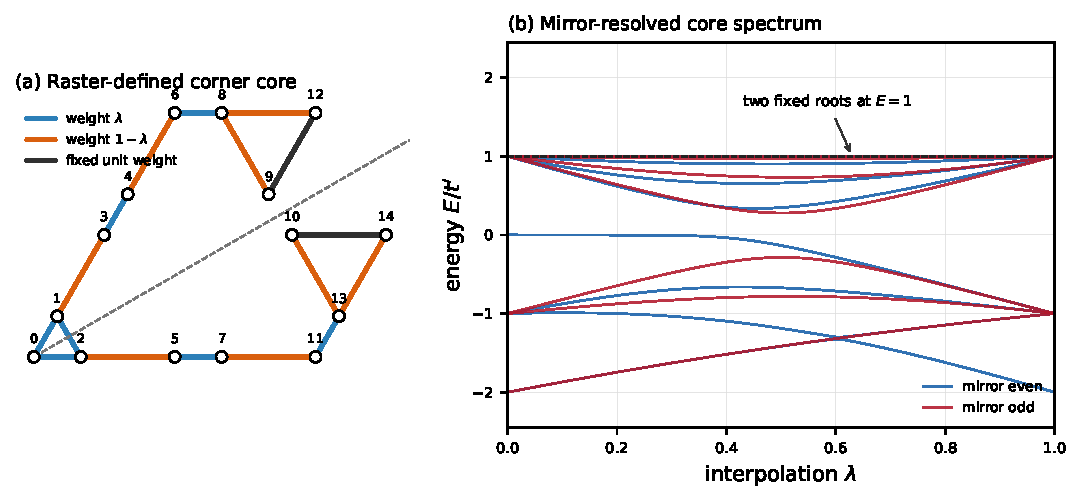
\includegraphics[width=0.96\textwidth]{fig_core_spectrum.pdf}
 \caption{(a) The complete 15-site invariant component specified by
 Eq.~\eqref{eq:edges}.  The dashed line is the reflection axis.
 (b) Spectrum obtained by diagonalizing the two reflection sectors; one
 $E=1$ root in each sector is fixed, while the remaining 13 roots are
 nonconstant.  Lines serve only as a visualization; the count follows from
 the exact polynomial argument in the text.  The vector-figure script was
 prepared with OpenAI Codex assistance and reads the exact edge certificate;
 the plotted eigenvalues were checked against the exact endpoint and
 factorization data.}
 \label{fig:core}
\end{figure*}

The endpoint factorizations supply a transparent first check.  At
$\lambda=0$ the component is an isolated site, four dimers, and two
triangles, whereas at $\lambda=1$ it is six dimers and one triangle.  Hence
\begin{align}
 \chi(E,0)&=E(E-1)^8(E+1)^4(E+2)^2,\label{eq:endpoint0}\\
 \chi(E,1)&=(E-1)^8(E+1)^6(E+2).\label{eq:endpoint1}
\end{align}

It remains to establish that Eq.~\eqref{eq:factorization} contains the
\emph{complete} interpolation-independent factor.  Write
$\chi(E,\lambda)=\sum_{m=0}^{12}c_m(E)\lambda^m$.  Exact fraction-free
elimination gives
\begin{equation}
 \gcd_{0\leq m\leq12}c_m(E)=(E-1)^2.
 \label{eq:gcd}
\end{equation}
Maximality can be checked from only two coefficients.  After division by
$(E-1)^2$, the coefficients of $\lambda^{11}$ and $\lambda^{12}$ are
\begin{equation}
 q_{11}(E)=50E^2-196E-22,\qquad q_{12}(E)=24E+4.
 \label{eq:witness}
\end{equation}
The sole root of $q_{12}$ is $-1/6$, while
$q_{11}(-1/6)=217/18$, so $q_{11}$ and $q_{12}$ are coprime.  No additional
polynomial in $E$ can therefore divide every $c_m$.

A $\lambda$-independent energy would contribute a factor of $E-E_0$ to
every coefficient of $\chi$.  Equations \eqref{eq:gcd} and
\eqref{eq:witness} consequently show that precisely two roots, counted with
generic algebraic multiplicity, are fixed throughout the interpolation.
The remaining $15-2=13$ roots are nonconstant.  This statement does not mean
that 13 distinct curves must be visually resolvable at every $\lambda$:
degeneracies with the flat edge and bulk bands can conceal a moving algebraic
root.

In the $N=20$ complete-cell triangular flake (630 sites), exact lattice
rotation gives three pairwise-disjoint copies of the component in
Eq.~\eqref{eq:edges}.  They contain all 21 bonds ramped on and all 24 bonds
ramped off; the exterior block is independent of $\lambda$ at $t=0$.
The nonconstant factor of the three-corner characteristic polynomial
therefore has degree
\begin{equation}
 3\times13=39,
\end{equation}
rather than the $3\times12=36$ inferred from the published count.

\section{Checks at finite intracell hopping}

The bivariate polynomial was obtained in exact integer/rational arithmetic
from the graph in Eq.~\eqref{eq:edges}, both directly and after mirror
reduction.  A separate implementation, sharing no polynomial code, evaluated
the characteristic polynomial by the Faddeev--LeVerrier recurrence at 16
integer values of $\lambda$ and reconstructed all coefficients by Newton
interpolation.  Two unused rational values, $\lambda=1/2$ and $-2/3$, agree
exactly.  As another check, at $\lambda=1/2$ one finds
$\operatorname{rank}(H_\lambda-I)=13$,
$\chi(-1,1/2)=27/256$, and
$\chi(-2,1/2)=-1112607/256$.  These evaluations independently exclude a
third fixed root among the energies common to the two endpoint spectra.

For context, the finite-$t$ calculation also sharpens how this local
rearrangement meets the edge spectrum.  On the balanced $N$-cell-side
termination, let $C=N(N+1)/2$.  For $N\geq6$, a square submatrix of the
$A\to B$ outgoing block is triangular and has exact determinant
\begin{equation}
 \det H_{BA}(\lambda)=(-1)^C t^{C-7}
 \big[(1-\lambda)t+\lambda t'\big]^7.
 \label{eq:minor}
\end{equation}
The cyclic partners obey the same formula.  Thus at $t=0.1$, $t'=1$, the
finite balanced flake has no exact eigenstate supported on only one
sublattice, even though its exponentially small boundary residual can mimic
a numerical kernel.

For $N=20$, exact rational inertia in the mirror-even $A_1$ and mirror-odd
$A_2$ sectors proves an order reversal of the 44th $A_1$ and 33rd $A_2$
levels (zero-based indices 43 and 32) between
\begin{equation}
 \lambda_L=\frac{7919395246780079}{10^{16}},\qquad
 \lambda_R=\frac{3959697623410039}{5\times10^{15}}.
 \label{eq:crossingbracket}
\end{equation}
Continuity and opposite mirror parity therefore imply at least one exact
crossing in this interval, near
$E=-0.554930413681\,t'$.  This is a finite-flake statement; neither crossing
uniqueness nor thermodynamic persistence follows.

The uniform edge outside the deformed core admits an evanescent ansatz
$(A,B,C)_{i,j}=r^iz^j(a,b,0)$.  Direct substitution gives
\begin{align}
 E^2&=t^2+t'^2+tt'(r+r^{-1}),\nonumber\\
 \frac{b}{a}&=-\frac{t+t'r}{E},\qquad
 z=-\frac{t(1+b/a)}{t'[1+(b/a)/r]}.
 \label{eq:transfer}
\end{align}
At the quoted crossing energy, the decaying solution has
$r=-0.1454530797104283$ and $z=-0.0587345561172001$.  The negative $r$
accounts for the observed alternating finite-size approach.  Its numerical
agreement with finite-flake ratios is evidence for the mechanism, not a proof
of a unique infinite-size secular root.

\section{Conclusion}

The local deformation of Ref.~\cite{Geschner2026} affects 13 nonconstant
algebraic roots per isolated corner component at $t=0$, not 12.  The
correction follows from a fully specified 15-site graph and an exact maximal
common-factor calculation.  It changes neither the removal of the corner
zero mode nor the obstructed-atomic-limit conclusion of the original paper.
It also supplies no general connectivity criterion, no bulk invariant, and
no thermodynamic phase-transition claim.

\section*{Data availability}

The exact graph and polynomial certificate, two independent reconstruction
scripts, the finite-crossing certificate, the edge-transfer data, the plotting
source, and environment specifications are included as ancillary files in the
submission package.

\begin{acknowledgments}
OpenAI Codex (model GPT-5.6-sol) assisted in a user-directed workflow with
primary-source comparison, exact-algebra and Python-code development,
independent computational checks, vector-figure preparation, and manuscript
drafting.  The central calculation was subjected to the independent exact
procedures described above.  The AI system is not an author.  Before any
submission, the named author must review the sources, reproduce and assess the
calculations, verify the figure and text, confirm permissions and the
disclosure, and take responsibility for the final manuscript.
\end{acknowledgments}

\bibliography{references}

\end{document}
